\chapter{Testy aplikacji}

\section{Wykorzystane technologie}

Do przetestowania aplikacji wykorzystano \textbf{Postmana} i \textbf{Lighthouse} \ref{tab:zestawienie_narzędzi}. Postman pozwoli sprawdzić czy zapytania oraz logika działają prawidłowo. Lighthouse pozwoli przeanalizować jakość strony internetowej


\section{Testowanie restowych zapytań przy pomocy Postmana}

Wykorzystując Postmana można na bieżąco monitorować stan aplikacji. Wykonując odpowiednie zapytania można sprawdzić w jaki sposób odpowiada aplikacja serwerowa na dane zapytanie. Ułatwia to pracę i wysyłanie zapytań z aplikacji klienckiej. Przetestowano każde z dostępnych zapytań zdefiniowane w tabeli \ref{tab:rest1} i \ref{tab:rest2}. Testowanie odbywało się na bieżąco z rozwojem systemu. Umożliwiło to szybką identyfikacje problemów.

\begin{figure}[htb]
  \centering
	\begin{tabular}{@{}llll@{}}
	a) & b) & c) & d) \\
	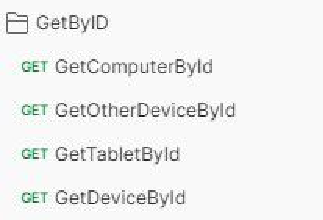
\includegraphics[width=0.17\linewidth]{rys06/struct/byid.pdf} & 
	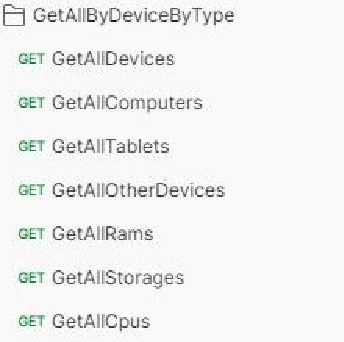
\includegraphics[width=0.17\linewidth]{rys06/struct/alldevices.pdf} & 
	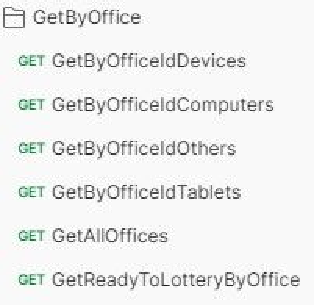
\includegraphics[width=0.17\linewidth]{rys06/struct/byOffice.pdf} & 
	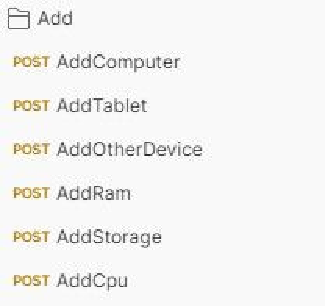
\includegraphics[width=0.17\linewidth]{rys06/struct/add.pdf} \\
 
	e) & f) & g) & h)\\
	
	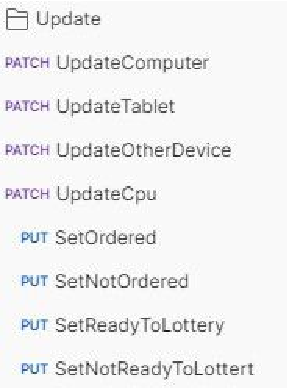
\includegraphics[width=0.17\linewidth]{rys06/struct/update.pdf} & 
	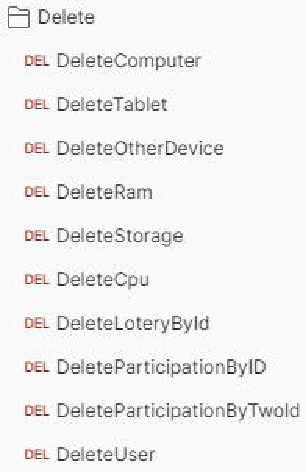
\includegraphics[width=0.17\linewidth]{rys06/struct/del.pdf} & 
	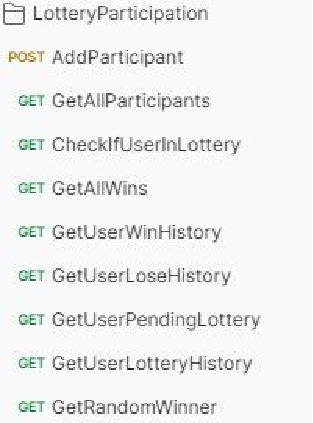
\includegraphics[width=0.17\linewidth]{rys06/struct/lottery.pdf} & 
	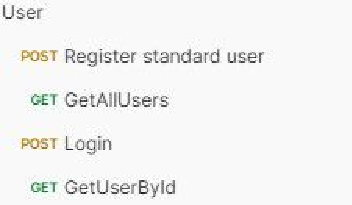
\includegraphics[width=0.17\linewidth]{rys06/struct/user.pdf} \\
 
 
	\end{tabular}
  \caption{Struktura testów a) po id, b) wszystkie urządzenia, c) sortowanie po biurze, d) dodawanie, e) aktualizacja, f) usuwanie, g) związane z loterią, h) związane z uzytkownikiem}
  \label{postmanStruct:label}
\end{figure}
\newpage

\subsection {Wybrane scenariusze testowe}


\subsubsection{Pobieranie informacji o sprzęcie}
Na scenariuszu testowym 1 \ref{getByIdTest:label} przetestowano pobieranie informacji o urządzeniu. Wykorzystując zapytanie \texttt{localhost:8080/devices/{id}} metodą GET uzyskano na scenariuszu testowym 1a i 1b status 200 OK. Wyświetlane informacje świadczą o poprawności działania funkcjonalności pobierania informacji o sprzęcie. W scenariuszu 1a zostały wyświetlone informacje o komputerze a w 1b o innym urządzeniu. Odpowiedź zapytania jest zależna od tego jakie urządzenie o zadanym ID ma typ. Możliwe jest coś takiego po wykorzystaniu schematu dziedziczenia które dostarcza unikalnych kluczy dal poszczególnych typów sprzętów. Więcej na ten temat napisano w rozdziale \ref{dzedziczenie_hibernate:label}.


\begin{figure}[htb]
  \centering
	\begin{tabular}{@{}ll@{}}
	a) & b) \\
  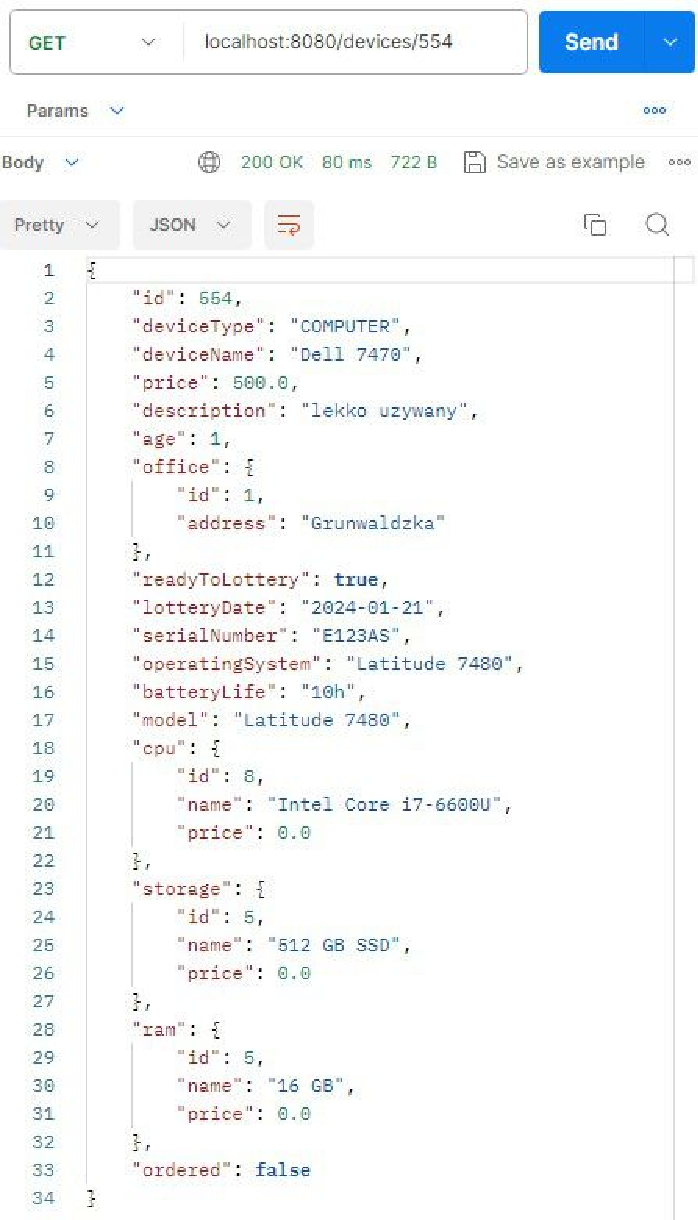
\includegraphics[width=0.5\textwidth]{rys06/postmanTest/compById.pdf} & 
	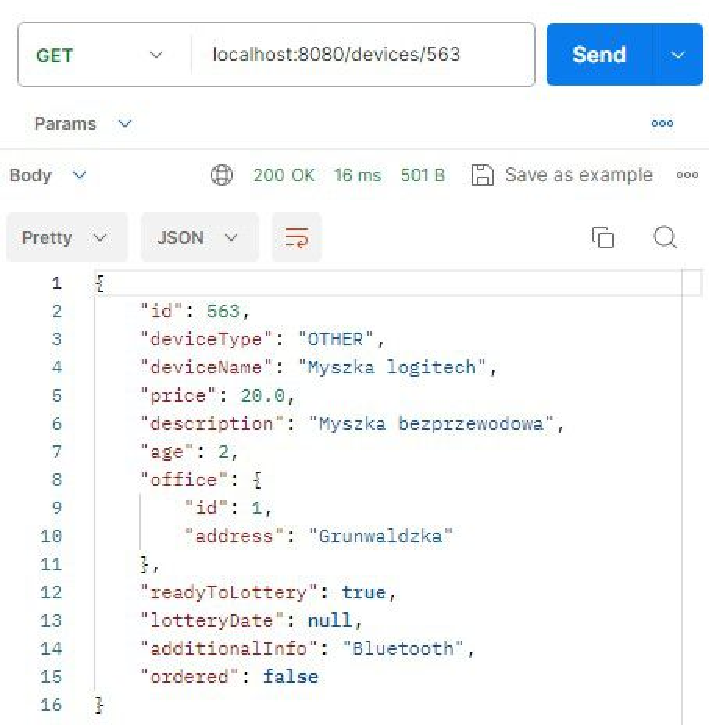
\includegraphics[width=0.5\textwidth]{rys06/postmanTest/otherById.pdf}
	\end{tabular}
  \caption{Scenariusz testowy 1,pobieranie informacji o urządzeniu, a) komputer, b) inne urządzenie}
  \label{getByIdTest:label}
\end{figure}



\subsubsection{Dodawanie i modyfikowanie urządzenia}
Na scenariuszu testowym 2 \ref{addModTest:label} najpierw dodano a potem zmodyfikowano dodane urządzenie. W obu przypadkach dane zostały wysłane jako JSON. W 2a po wysłaniu żądania metodą POST uzyskano status HTTP 201 Created. Oznacza to że urządzenie zostało poprawnie dodane do systemu. W dolnej części 2a widać jakie urządzenie zostało stworzone i jakie ma parametry. Scenariusz 2b modyfikuje utworzone w 2a urządzenie.Potrzebuje do tego oprócz danych zmieniających sprzęt ID urządzenia. ID jest przekazywane przez ścieżkę url. Możliwa jest modyfikacja pól w ten sposób by były miały wartość null. Skorzystano tutaj z metody PATCH która modyfikuje istniejący element.

\begin{figure}[htb]
  \centering
	\begin{tabular}{@{}ll@{}}
	a) & b) \\
  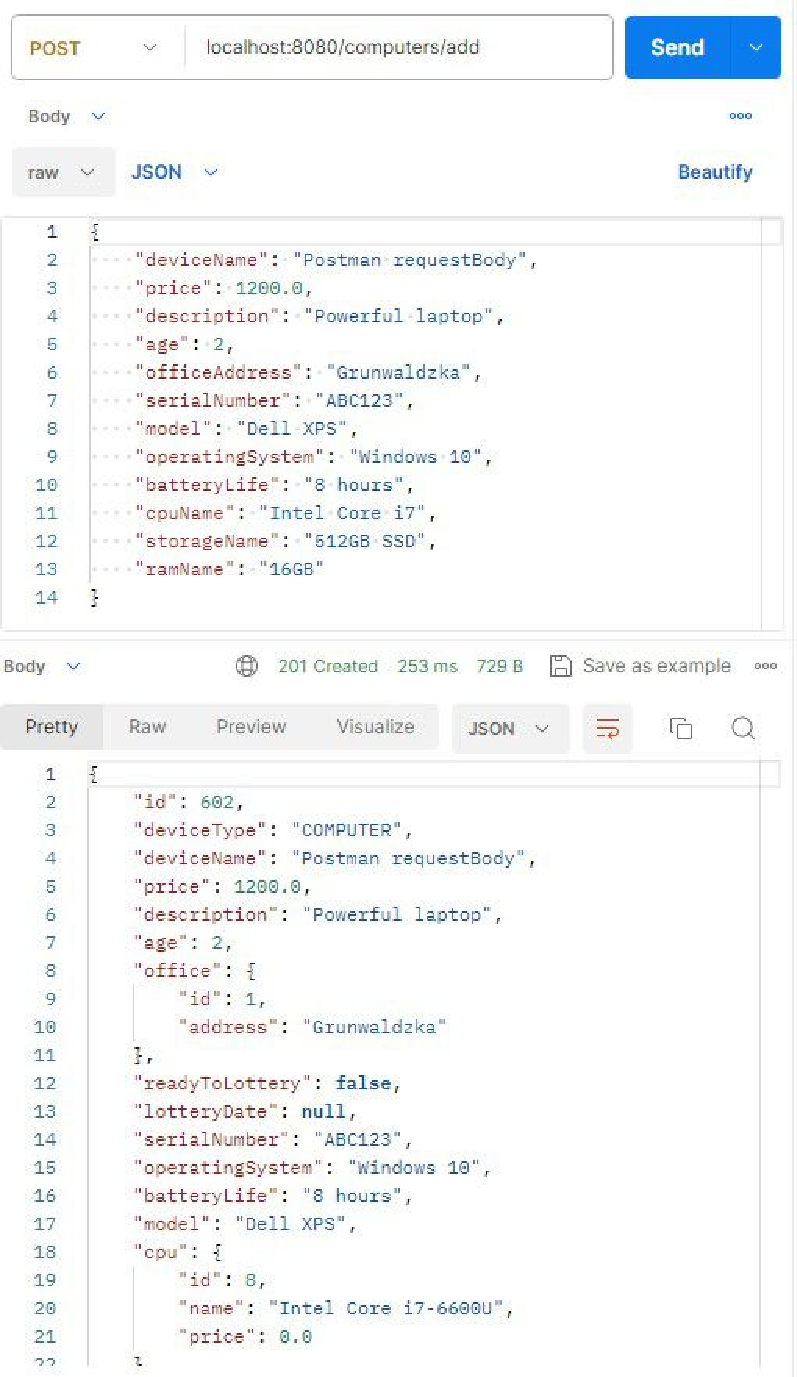
\includegraphics[width=0.45\textwidth]{rys06/postmanTest/addComp.pdf} & 
	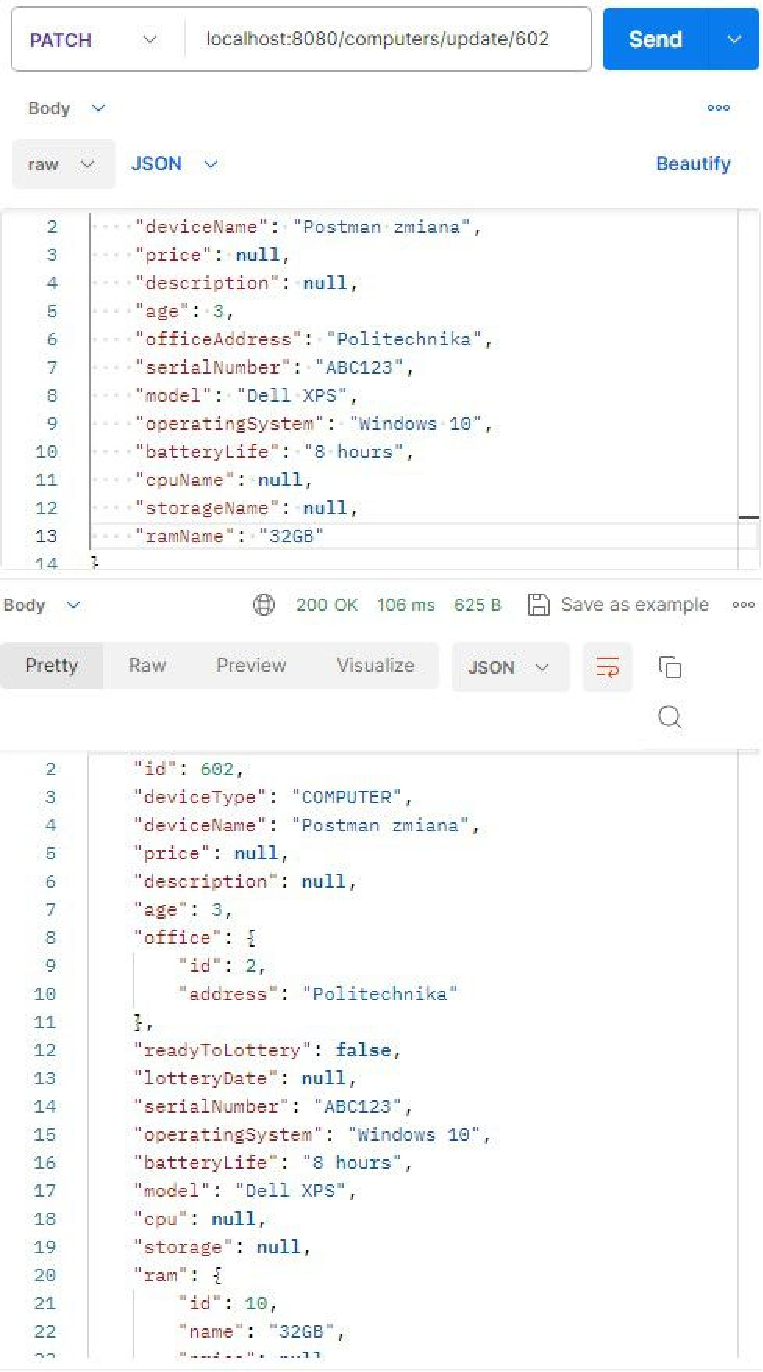
\includegraphics[width=0.45\textwidth]{rys06/postmanTest/patch.pdf}
	\end{tabular}
  \caption{Scenariusz testowy 2,Dodawanie i modyfikowanie komputera, a) dodawanie, b) modyfikacja}
  \label{addModTest:label}
\end{figure}



\subsubsection{Usuwanie urządzenia}
W scenariuszu testowym 3 \ref{deleteTest:label} pokazano w jaki sposób jest usuwane urządzenie. Do usunięcia urządzenia potrzebne jest ID, które przekazywane jest przez ścieżkę url. Po skorzystaniu z metody DELETE uzyskiwany jest status http 200 OK, który oznacza, że urządzenie zostało pomyślnie usunięte.


\begin{figure}[h]
		\centering
    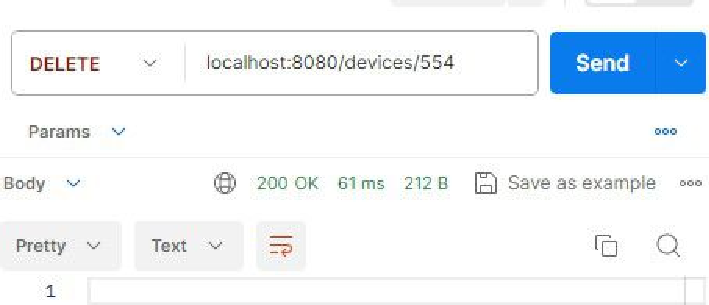
\includegraphics[width=0.45\linewidth]{rys06/postmanTest/delete.pdf}
    \caption{Scenariusz testowy 3, Usuwanie urządzenia po ID}
    \label{deleteTest:label}
\end{figure}


\subsubsection{Losowanie zwycięzcy}

Jedną z głównych funkcjonalności aplikacji jest przeprowadzenie losowania. Scenariusz testowy 3 \ref{winnerTest:label} pokazuje w jaki sposób jest przeprowadzane losowanie. W przypadku kiedy loteria posiada zapisanych użytkowników, losowany jest zwycięzca, jako status HTTP uzyskiwany jest 200 OK. W scenariuszu 3b pokazano przypadek kiedy na loterię nie został zapisany żaden pracownik lub loteria nie została otworzona. Wtedy status HTTP jest 204 No Content. 


\begin{figure}[htb]
  \centering
	\begin{tabular}{@{}ll@{}}
	a) & b) \\
  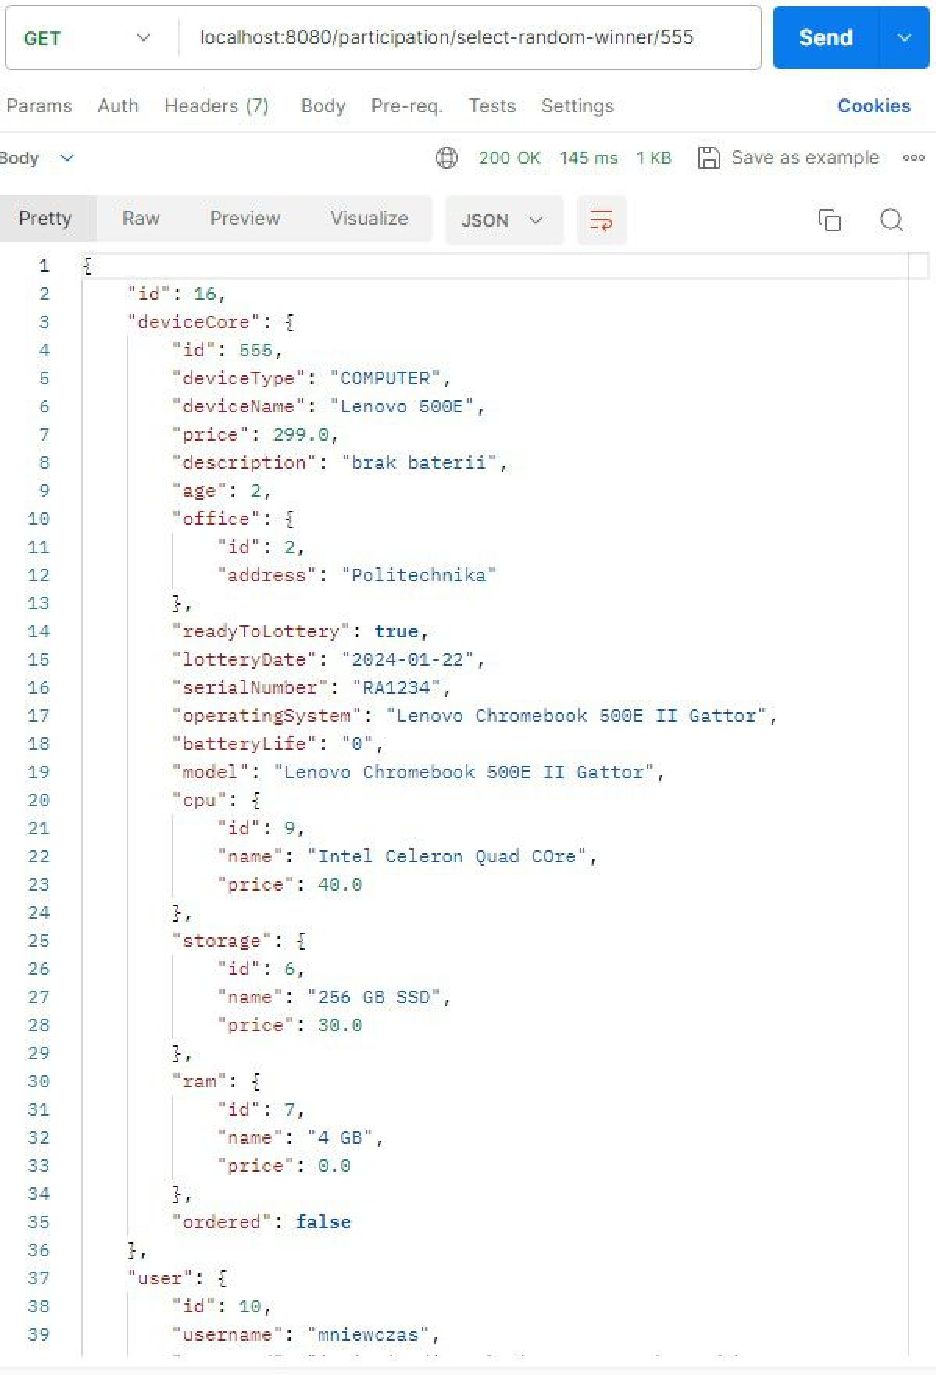
\includegraphics[width=0.5\textwidth]{rys06/postmanTest/winner.pdf} & 
	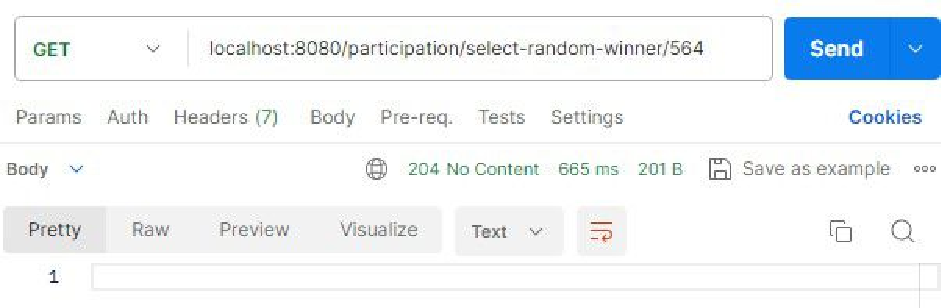
\includegraphics[width=0.5\textwidth]{rys06/postmanTest/badWinner.pdf}
	\end{tabular}
  \caption{Scenariusz testowy 3,Losowanie zwycięzcy, a) powodzenie, b) niepowodzenie}
  \label{winnerTest:label}
\end{figure}

\newpage
\subsubsection{Rejestracja użytkownika}
Scenariusz testowy 4 \ref{registerTest:label} pokazuje jak działa rejestracja użytkownika. Po utworzeniu takiego użytkownika zwracany jest status HTTP 201 Created. Użytkownik taki zapisywane hasło ma w postaci zaszyfrowanej.

\begin{figure}[h]
		\centering
    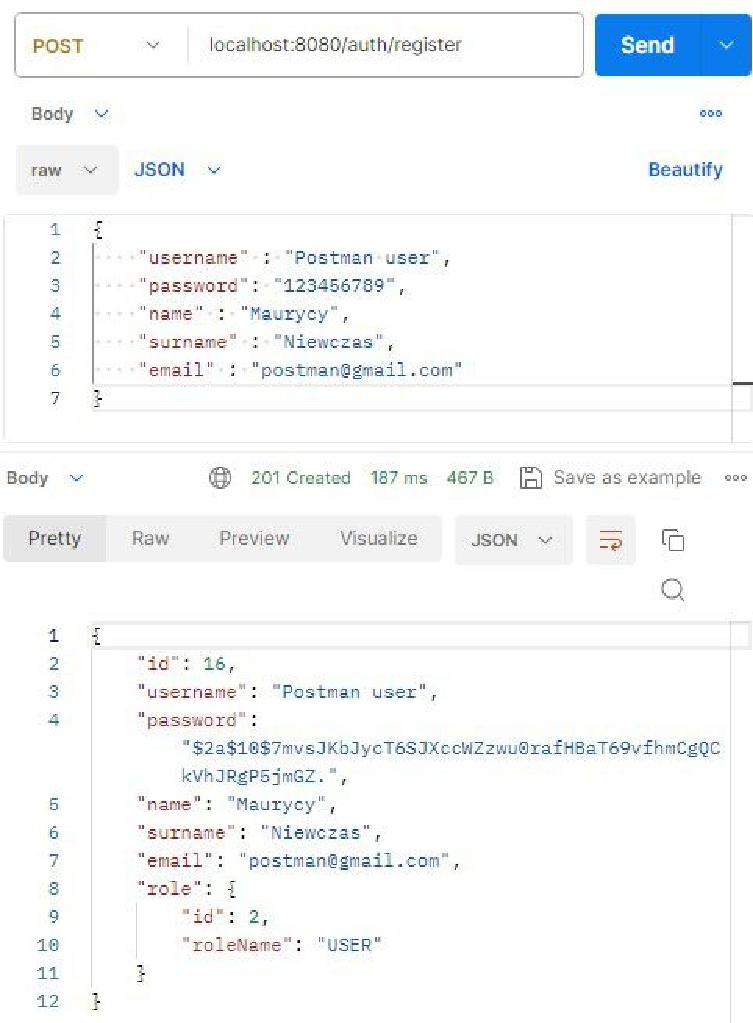
\includegraphics[width=0.7\linewidth]{rys06/postmanTest/register.pdf}
    \caption{Scenariusz testowy 4, Rejestracja użytkownika}
    \label{registerTest:label}
\end{figure}

\newpage
\section{Testowanie jakości strony internetowej systemu przy użyciu Lighthouse}

Wykorzystanie Lighthouse \ref{tab:zestawienie_narzędzi} pozwala na zbadanie wydajności, dostępności i dobrych praktyk strony internetowej. Testowany widok był strony domowej, ponieważ na niej dzieje się większość logiki systemu. Testowanie odbyło się w dwóch wariantach: strony domowej administratora i strony domowej pracownika \ref{lh:label}

\begin{figure}[htb]
  \centering
	\begin{tabular}{@{}ll@{}}
	a) & b) \\
  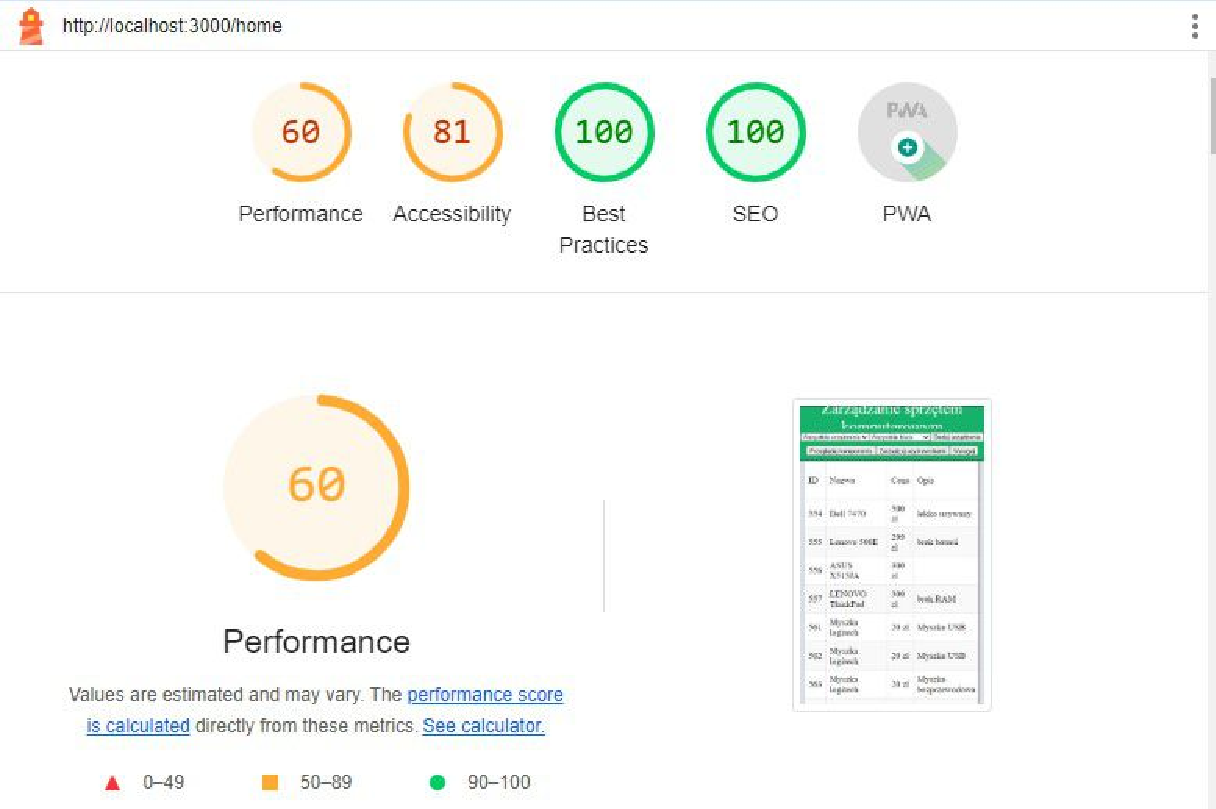
\includegraphics[width=0.5\textwidth]{rys06/lighthouse/adminLightHouse.pdf} & 
	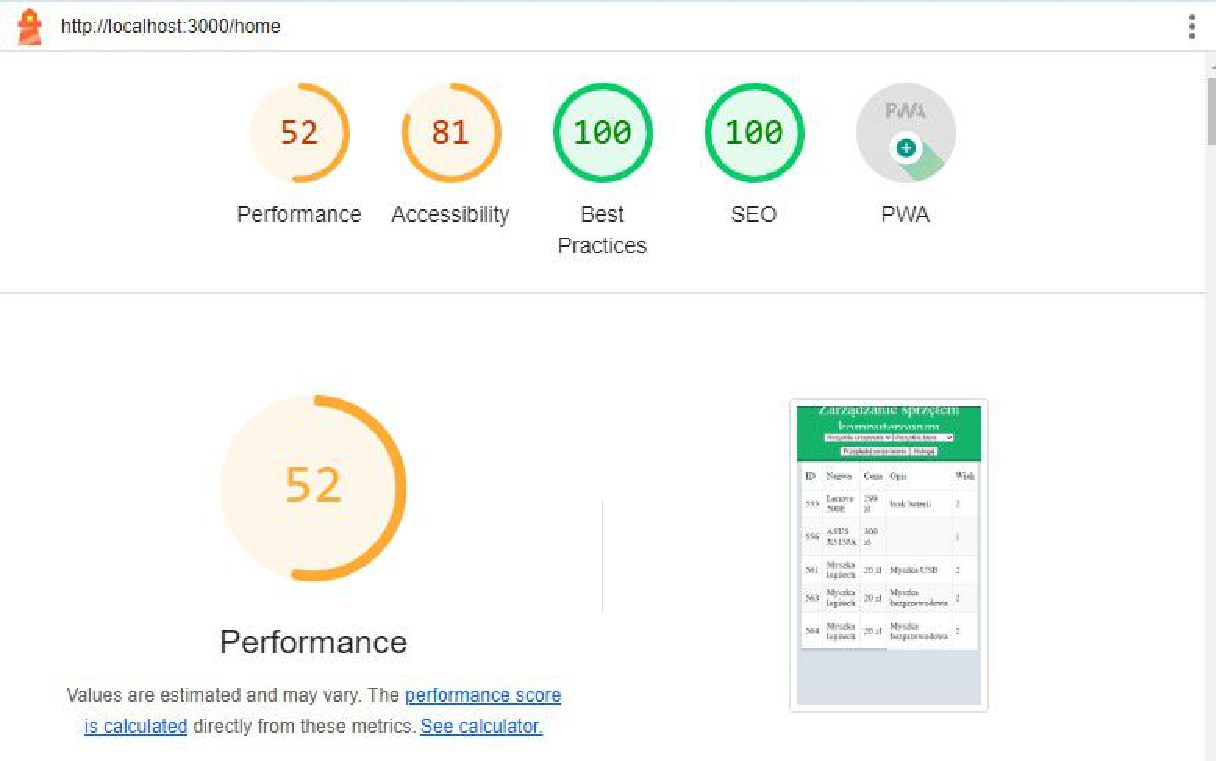
\includegraphics[width=0.5\textwidth]{rys06/lighthouse/workerLightHouse.pdf}
	\end{tabular}
  \caption{Test Lighthouse strony domowej, a) administratora, b) pracownika}
  \label{lh:label}
\end{figure}

Wnioskując z testu widok aplikacji ma satysfakcjonujące parametry.
\begin{itemize}
\item \textbf{Wydajność (Performance)} jest na średnim poziomie. Pokazuje to że aplikacja mogła by być bardziej zoptymalizowana pod względem wydajności
\item \textbf{Dostępność (Accessibility} jest na wysokim poziomie. Oznacza to, że osoby z różnymi niepełnosprawnościami nie miałyby większego problemu z posługiwaniem się aplikacją. Jednak tutaj jest możliwość optymalizacji by osiągnąć większy stopień zadowolenia tych użytkowników.
\item \textbf{Dobre praktyki (Best Practices)} pokazuje, że test przeszedł test dobrych praktyk i storn a jest zgodna ze standardami.
\item \textbf{SEO} - Pokazuje, że strona jest zoptymalizowana pod kątem wyszukiwarek internetowych
\end{itemize}

